\documentclass[twocolumn]{aastex62}


\DeclareGraphicsExtensions{.jpg,.pdf,.png,.eps,.ps}

\def\jcap{J. of Cosm. \& Astropart. Phys.}

\def\tbd{\textcolor{red}{TBD}}

\usepackage{amsmath,amsbsy}
%% Definitions of useful commands      
\newcommand{\lcdm}{\ensuremath{\Lambda\mathrm{CDM}}} 
\newcommand*\Bell{\ensuremath{\boldsymbol\ell}}
 \newcommand{\nhat}{\ensuremath{\mathbf{\hat{n}}}}
 \newcommand{\sigT}{\mbox{$\sigma_{\mbox{\tiny T}}$}}
 \newcommand{\Tcmb}{\mbox{$T_{\mbox{\tiny CMB}}$}}
 \newcommand{\sz}{Sunyaev-Zel'dovich}
 \newcommand{\sze}{Sunyaev-Zel'dovich Effect}
 \newcommand{\neff}{\ensuremath{N_\mathrm{eff}}\xspace}
 \newcommand{\yhe}{\ensuremath{Y_p}}
 \newcommand{\As}{\ensuremath{A_s}}
 \newcommand{\deltaR}{\ensuremath{\Delta_R^2}}
 \newcommand{\nrun}{\ensuremath{dn_s/d\ln k}\xspace}
 \newcommand{\alens}{\ensuremath{A_{L}}}
 \newcommand{\ns}{\ensuremath{n_{s}}}
 \newcommand{\ho}{\ensuremath{H_{0}}\xspace}
 \newcommand{\LCDM}{\mbox{$\Lambda$CDM}\xspace}
 \newcommand{\muksq}{\ensuremath{\mu{\rm K}^2}}
 \newcommand{\sumnu}{\ensuremath{\Sigma m_\nu}\xspace}
 \renewcommand{\vec}[1]{\mathbf{#1}}
 \newcommand{\Lk}{\mathcal{L}}
 \def\be{\begin{equation}}
\def\ee{\end{equation}}
\def\ba{\begin{eqnarray}}
\def\ea{\end{eqnarray}}
 
% experiments
 \newcommand{\wmap}{\textit{WMAP}}
 \newcommand{\wseven}{\textit{WMAP}7}
 \newcommand{\wnine}{\textit{WMAP}9}
 \newcommand{\sptpol}{SPTpol}
  \newcommand{\sptsz}{SPT-SZ}
 \newcommand{\planck}{\textit{Planck}}
 \newcommand{\polarbear}{POLARBEAR}
 \newcommand{\bicep}{BICEP2}
 \newcommand{\keck}{KECK Array}
 \hyphenation{BICEP}
 \hyphenation{POLAR-BEAR}
 
 % Referee comments
 \def\RC{\color{ForestGreen}}
 

 
\begin{document}

%\title{Simulating Galactic Dust with Deep Convolutional Generative Adversarial Networks}
\title{Cleaning our own Dust: Simulating and Separating Galactic Dust Foregrounds with Convolutional Networks}
\author{K. Aylor}
\affiliation{Department of Physics, University of California, Davis, CA, USA 95616}
\author{ M. Haq}
\author{L. Knox }
\affiliation{Department of Physics, University of California, Davis, CA, USA 95616}
\author{Y. Hezaveh }
\affiliation{Department of Physics, Stanford University, Stanford, CA, USA 94305}


 \email{kmaylor@ucdavis.edu}

\begin{abstract}
Measuring the cosmic microwave background (CMB) with greater detail is the focus of several upcoming experiments. However, the primary signal of interest is partially contaminated by thermal emission from interstellar dust grains. Separating this foreground emission, and
quantifying the uncertainty in the CMB map due to errors in foreground separation, are
important for avoiding biases in scientific conclusions to be made from the CMB maps. Our ability to quantify such uncertainty is limited by our lack of a model for the statistical
distribution of the dust foreground. To overcome this challenge we use a Deep Convolutional Generative Adversarial Network (DCGAN) in order to generate sample dust foreground skies from an underlying probability distribution. The input data is a set of dust maps inferred from observations by the Planck satellite. A DCGAN is uniquely suited for such unsupervised learning tasks where we have no a priori knowledge of the underlying statistical distribution.
\end{abstract}

\keywords{deep convolutional generative adversarial networks, cosmic microwave background, galactic dust simulations}



\section{Introduction}
1: Separating dust from CMB important for next stage of experiment
1a: Can be done with neural networks
2: Better foreground removal depends on a statistical model of the dust
2a: Current simulation methods rely on replicating low ell spectra and making assumptions about remaining structure
2b: Current separation methods rely on assumptions about spatial and frequency dependence
3: what are neural networks
4: how we plan to use them
4a: gan for simulations
4b: autoencoder to remove foregrounds
5: section summary


Measurements of the cosmic microwave background (CMB) have provided the most sensitive probe of the initial state of the universe, its evolution, and contents. In recent years major milestones have been reached with the completion of the SPT-SZ, Planck, and ACT surveys and we have been able to pin down several cosmological parameters to great precision. Much work has been completed in moving towards the next stage of experiments (SPT-3G, ADVACT, and S4) where measurements of even smaller angular scales will be pushed to the sample variance limit. The success of these future experiments will rely on being able to accurately remove the foreground signal from the the CMB. In this paper we present methods relying on deep convolutional neural networks to not only generate map level simulations of foregrounds but to also remove the interfering signal from CMB maps.

Talk more about dust here and how it is currently modeled and removed.

Neural networks are a form of machine learning, the development of which was loosely based on how signals are transmitted through a nervous system. In general neural networks approximate a target function as a series of affine and non-linear transformations, the weights of which are learned during a training process known as backpropagation; the error from a loss function is used to adjust the model weights via stochastic gradient descent or some other optimization algorithm. Over the last decade neural networks have become increasingly more popular as a method for performing classification and regression as they have been shown to be universal approximators \citep{csaji01}. 

Developments in modeling via neural networks and the availability of powerful computation resources open up a new approach to conducting cosmological analyses. In particular they can be used to create highly accurate simulations based on the data without trying to emulate a particular summary statistic and perform map level component separation without relying on a particular spatial or frequency dependence.  In Section 2 we present our method for developing interstellar dust simulations using a Deep Convolutional Generative Adversarial Network and in Section 3 we discuss the results of the training. We conclude with a discussion on future work utilizing our simulations and a second type of neural network to separate CMB from foregrounds.


\section{Generative Adversarial Network}

A Generative Adversarial Network (GAN) is a form of unsupervised machine learning which attempts to model a generating function which can create samples from a desired distribution \citep{goodfellow14}. 
A GAN consists of two sub-models, a discriminator and a generator, each with their own sets of weights that are to be optimized.
The discriminator is optimized to detect samples from $P$, the distribution which we desire to emulate, and the generator is optimized to create samples from $P$.
During the training process the discriminator is shown labeled samples from $P$ and from the generator, as the discriminator improves at detecting samples from $P$ the generator must improve at creating samples belonging to $P$ to minimize its own loss function. Training proceeds until the generator's output distribution has converged to $P$.
For the case of generating $N\times M$ pixel images a Deep Convolutional GAN (DCGAN), first presented in \cite{radford15}, has proven to be effective. In this architecture the generator $\rm{G}(z)$ maps $z$, a random vector from $Z$, to $P$ in $\mathbb{R}^{N\times M}$ through a series of upsamplings via strided convolutions. 
The generator then allows one to sample from $P$ as $Z$ is chosen to be a distribution where it is known how to produce samples i.e. a Gaussian distribution.

In our case $P$ is the thermal distribution of interstellar dust across the sky.
A DCGAN allows us to generate simulations of dust intensity maps based on the actual measured distribution instead of relying on a particular set of assumptions. 
As we only have one sky to measure we are limited in our ability to measure samples from $P$ and instead focus on a subset of $P$, patches of sky with approximately 1\% coverage. 
The primary reason for choosing 1\% versus some other size is this coverage reduces the computational power needed to develop a model while still covering angular scales of interest.

\subsection{The Dataset}
We formed our training dataset from the \planck\ 343GHz GNILC thermal dust map \citep{planck16-48}. The map was cut into overlapping patches of approximately 1\% sky coverage by selecting a $20^{\rm{o}} \times 20^{\rm{o}}$ region centered on a great circle (allowing us to use the flat sky approximation) using $\it{healpy}$ \citep{gorski05}.  One can envision our sampling process as shifting the center of a patch at a given longitude and latitude, $(\phi,\theta)$, to  $(\phi+s/cos(\theta),\theta+s)$, where $s$ is the step size,  and selecting a $20^{\rm{o}} \times 20^{\rm{o}}$ region centered on a great circle going through the new center. The factor of $1/cos(\theta)$ is included in the longitude step size to avoid over sampling of the poles. We also exclude the galactic plane by only sampling regions 15 degrees above and below the plane. This is done to ease convergence by reducing the dynamic range of the temperature. For a more detailed analysis the galactic plane could be included. For $s=5$ we created roughly 1000 map cuts.  We chose a resolution of $900\times900$ pixels for each image to ensure good coverage when mapping the images back to the sphere. The average angular size of an individual pixel is less than two arcmin, which is smaller than the \planck\ beam width. Before training we normalize the dataset to the range $[-1,1]$.

\subsection{Network Architecture}
We base the architecture of our discriminator and generator on the guidelines presented in \cite{radford15} with several exceptions.
We replaced all transpose convolution layers in the generator with a bi-linear upsampling followed by a convolutional layer with a stride of one.
We found this method lead to better convergence in the generator by eliminating the checkerboarding artifact that can be found with transpose convolution layers \citep{odena16}.
The generator recieves a 64-dimensional vector drawn from $\mathcal{N}(0,1)$ as input, which is then processed through a densely connected layer and reshaped into \tbd $\tbd \times \tbd$ maps.
This is followed by \tbd layers of upsampling and convolution which result in a single map.
This map is then cut down to $900\times900$ pixels in the final layer. 
After each linearity in the generator we apply a LeakyReLU activation, with $\alpha = 0.2$, except in the final layer where we apply a hyperbolic-tangent (tanh) activation.
We also apply Batch Normalization, with a momentum of 0.9, after each activation layer except the final one. In Table \ref{tab:gan_layers} we list the structure of the generator.

\begin{table}[ht]
\centering

 \begin{tabular}{ c c c c }
 \hline\hline
  Operation & Output & Hyperparameters \rule{0pt}{2.5ex} \\ [0.5ex]
 \hline
  Linear & $6\times 6\times 256$  & \rule{0pt}{3.0ex} \\
  Leaky ReLU & $6\times 6\times 256$ & $\alpha=0.2$ \\
  Batch Normalization & $6\times 6\times 256$ & $\rm{momentum} = 0.9$ \\  
  Up Sampling & $30\times 30\times 128$ & bi-linear \\ 
  Convolution & $30\times 30\times 128$ &  \\
  Leaky ReLU & $30\times 30\times 128$ & $\alpha=0.2$ \\
  Batch Normalization & $30\times 30\times 128$ & $\rm{momentum} = 0.9$ \\  
  Up Sampling & $120\times 120\times 64$ & bi-linear \\ 
  Convolution & $120\times 120\times 64$ &  \\
  Leaky ReLU & $120\times 120\times 64$ & $\alpha=0.2$ \\ 
  Batch Normalization & $120\times 120\times 64$ & $\rm{momentum} = 0.9$ \\  
  Up Sampling & $480\times 480\times 32$ & bi-linear \\ 
  Convolution & $480\times 480\times 32$ &  \\
  Leaky ReLU & $480\times 480\times 32$ & $\alpha=0.2$ \\ 
  Batch Normalization & $480\times 480\times 32$ & $\rm{momentum} = 0.9$ \\  
  Up Sampling & $960\times 960\times 1$ & bi-linear \\ 
  Convolution & $960\times 960\times 1$ &  \\
  Tanh & $960\times 960\times 1$ & $\alpha=0.2$ \\
  Crop & $900\times 900\times 1$ &  \\ [1ex]
 \hline
\end{tabular}
\caption{The output structure and relevant hyperparameters for each layer in the generator.}
\label{tab:gan_layers}
\end{table}

For the discriminator we use the same number of feature maps. The upsampling and convolution steps in the generator are replaced by a convolution in the discriminator with a stride equal to the upsampling of the corresponding layer. After each convolution we again apply a LeakyReLU activation and Batch Normalization with the same alpha and momentum as in the generator. The feature maps are then flattened into a 1-dimensional vector and passed through a densely connected layer with a sigmoid activation function.

\subsection{Training}
For the discriminator we used a binary cross entropy loss function and the Adam optimizer with the learning rate set to $2\times10^{-4}$ and $\beta_1=0.5$. These are the same settings suggested in \cite{radford15}. We initialize the weights of the network from a truncated normal distribution with a standard deviation of 0.2. Training is done in batches of 32 maps. First the discriminator is trained on 16 real and 16 fake images (produced by the current state of the generator), the images' labels are also swapped with 1\% probability. Next the generator is given 32 random noise vectors and the output from the generator is passed to the discriminator to calculate the loss. We repeat this process until we have reached a desired level of convergence.






\section{Results}

To determine if the generator produces samples that are statistically consistent with the dataset, we follow the procedure presented in \cite{mustafa17}. We focus on three summary statistics, the pixel intensity, power spectra, and Minkowski functional distributions. The first two statistics capture the first and second order information while the third is sensitive to  non-Gaussianities (the expected distribution of dust is highly non-Gaussian). To quantify the agreement between the summary statistics of the generated and real maps we rely on the Kolmogorov-Smirnov (KS) test; a large p-value means we cannot reject the null-hypothesis that the generated maps are drawn from the same distribution as the real maps.

In Figure \ref{fig:pix_int} we show the distribution of pixel intensities over the entire set of real maps and 1000 generated maps. We chose to use 1000 generated samples as the summary statistics for larger numbers of samples showed little difference. From Figure \ref{fig:pix_int} we see the generator has learned the distribution of pixel intensities and we find a KS p-value of \tbd. The largest discrepancy between the distributions appears at the tails and most predominantly at the higher intensities. This is to be expected as a generator will have more difficulty learning this region simply due to the low rate at which such pixels are seen during training. 



\begin{figure}
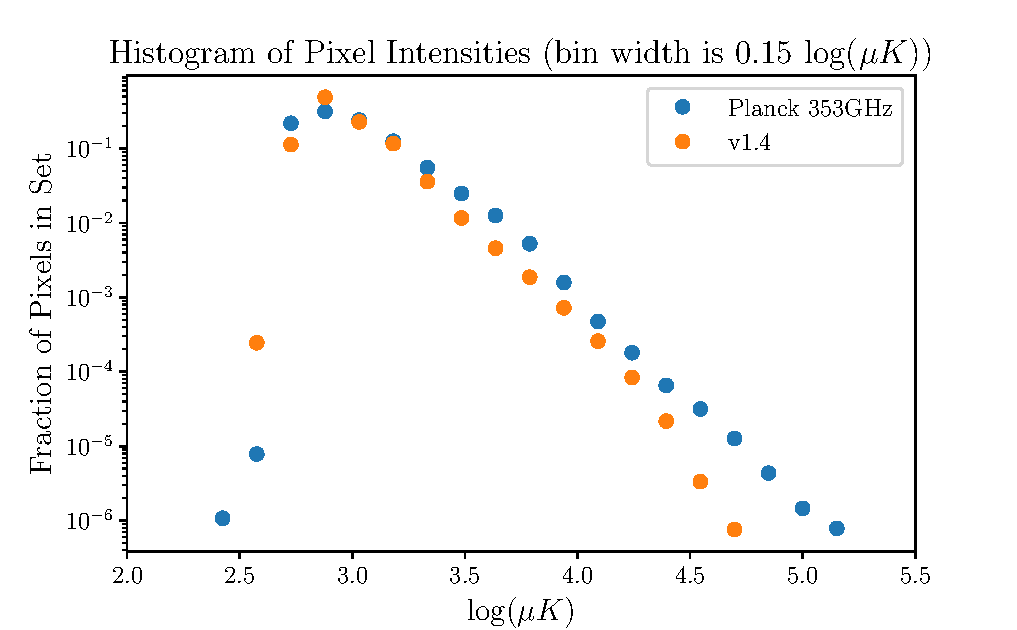
\includegraphics[width = .5\textwidth]{HistPixIntensity.pdf}
\caption{The pixel intensity distribution for 1000 real and 1000 generated maps. We found a p-value of \tbd for the Kolmogorov-Smirnov test.}
\label{fig:pix_int}
\end{figure}

The statistic of primary interest of dust intensity maps is the angular power spectrum. The power spectrum of a temperature map is the variance in the temperature at different scales; it is the most informative statistic of the CMB and measurements of it have resulted in the tightest constraints on cosmological models. The  dust is an additive  component to the signal of a measured power spectrum and accurate modeling of the dust power spectrum is needed to provide the best possible estimates of cosmological parameters in future experiments. 

The angular scale of our maps allow us to take the flat sky approximation and we calculate power spectra from 2-D Fourier modes instead of spherical harmonics. In Figure \ref{fig:power} we show the mean and 68\% intervals for the real and generated sets. For  each bin we calculate KS p-values ranging from [\tbd,\tbd]. In Figure \ref{fig:powerhist} we show the distribution for three different  scales. Our generator has clearly replicated the distribution from the real set of maps.

\begin{figure}
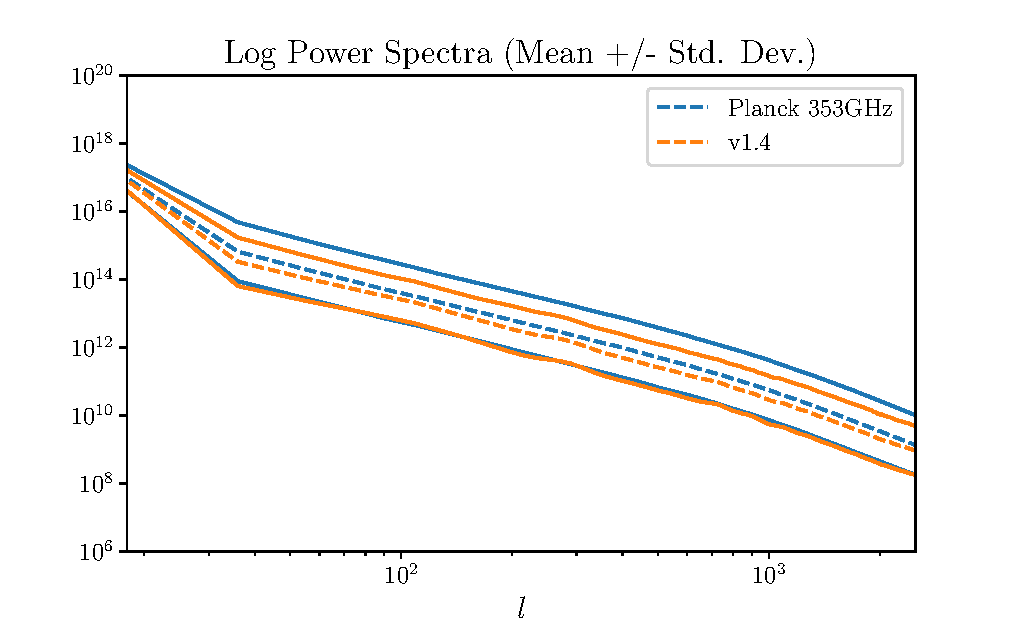
\includegraphics[width = .5\textwidth]{LogPowerSpectra.pdf}
\caption{The distribution of power spectra of the real and generated dust intensity maps. The dashed curves are the mean of the distribution and the solid curves mark the 68\% confidence intervals. The p-values for the individual $C_{\ell}$ bins range from \tbd to \tbd. }
\label{fig:power}
\end{figure}

\begin{figure*}[!tbh]
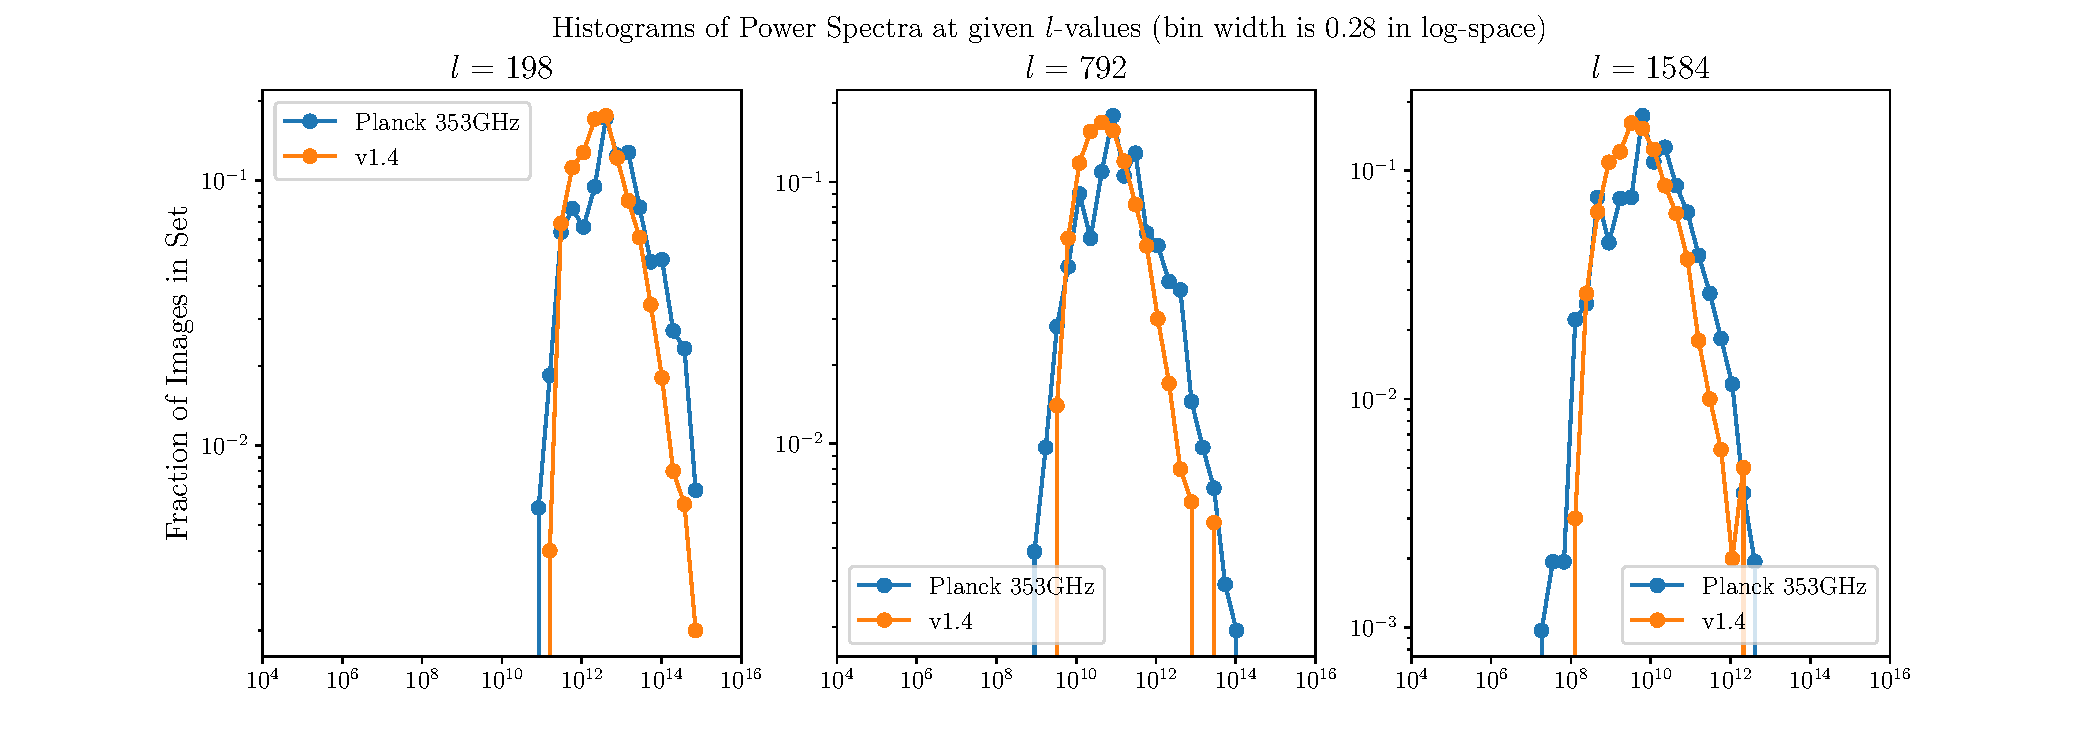
\includegraphics[width = \textwidth]{HistPowerSpectraSlices.pdf}
\caption{The distributions of the $C_{\ell}$ for three separate bins at $\ell=\tbd,\tbd,\tbd$. From left to right the KS p-values are \tbd,\tbd, and \tbd}
\label{fig:powerhist}
\end{figure*}

The dust maps contain non-Gaussian information which is not captured by the first and second order statistics. In order to compare the non-Gaussian features of the real and generated sets we use the Minkowski Functionals $V_0$, $V_1$, and $V_2$, which respectively measure the area of the foreground, the perimeter of the foreground, and the connectivity of the foreground for various thresholds.  In Figure \ref{fig:mink} we show the functionals evaluated at 32 different threshold values after normalizing the maps to the range [-1,1]. Again we find our generator has learned the correct distribution as evidenced by KS p-values ranging from [\tbd,\tbd]. 

\begin{figure*}[!tbh]
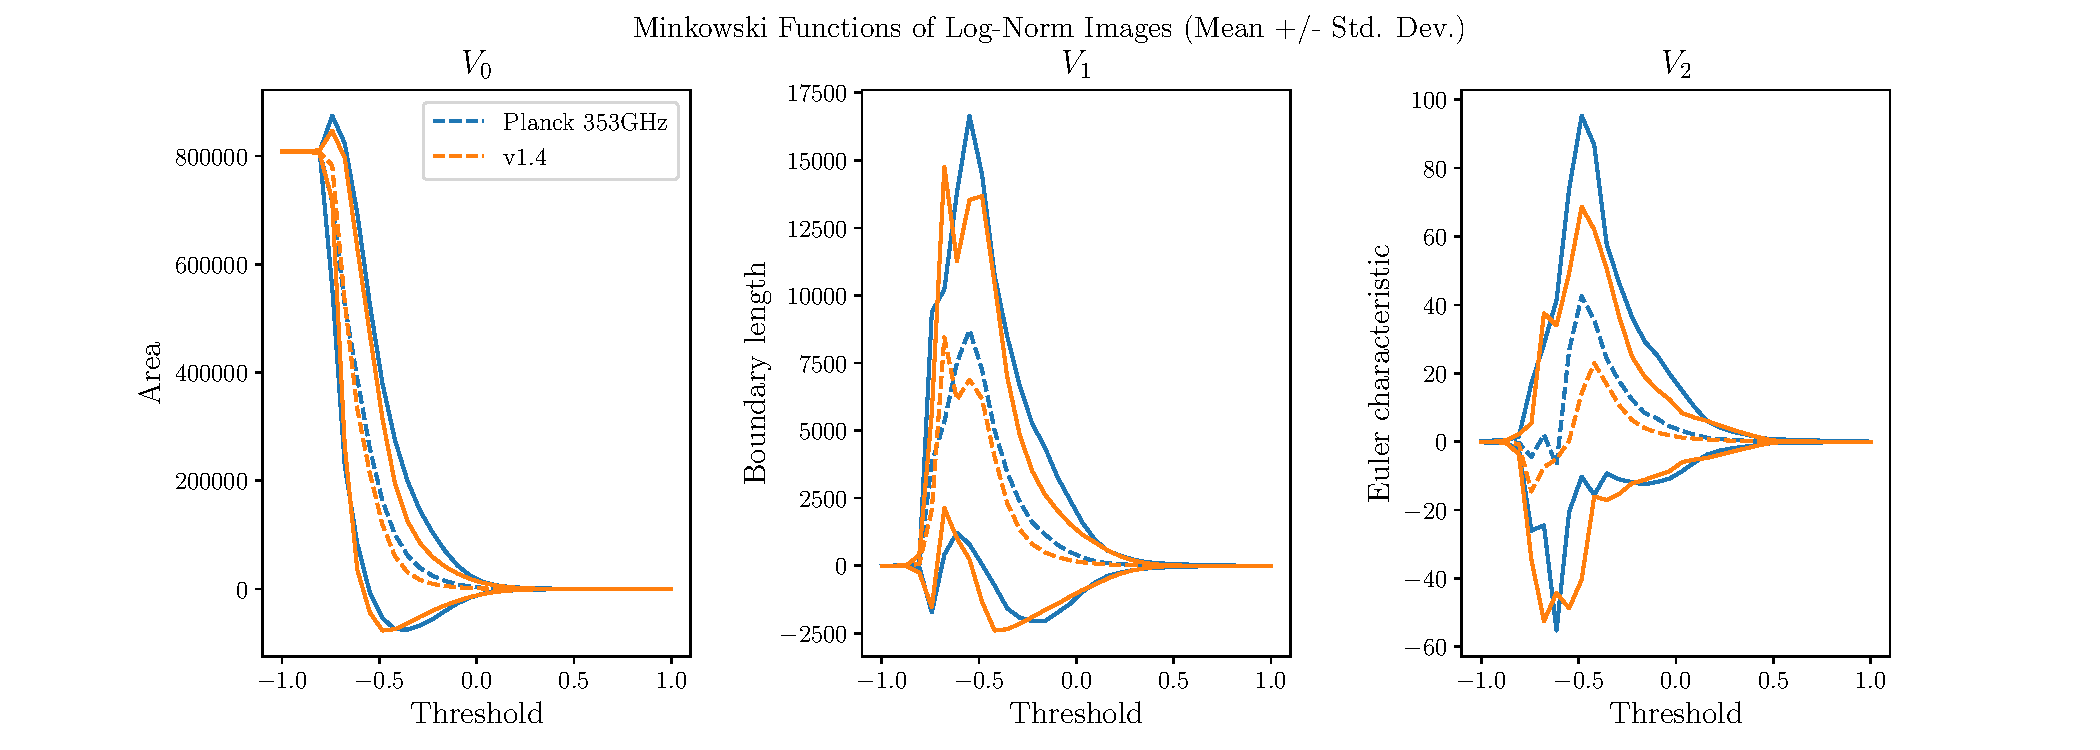
\includegraphics[width = \textwidth]{MinkowskiFunctionals.pdf}
\caption{The Minkowski functionals for the real and generated intensity maps. The dashed curves are the mean of the distribution and the solid curves mark the 68\% confidence intervals. The p-values for the individual $C_{\ell}$ bins range from \tbd to \tbd.}
\label{fig:mink}
\end{figure*}

Generally validation of a neural network's predictions or outputs is done against a subset of the training data to test if a model has overfit the data or generalized well. However we do not follow this practice for three reasons. First, we only have roughly 1000 images in our dataset, splitting this into a training and validation set would result in too few samples for either set. Second, the process of mapping portions of the sky to a Cartesian plane without overlap would leave portions of the full sky unsampled and significantly reduce the size of our dataset. We therefore rely on maps with some overlap. Even if we split this set into a training and validation set a significant amount of correlation would remain due to the overlap of the individual maps. Finally, since we are not working with a classification problem we are not concerned about generalizing, as we are trying to produce samples from a specific distribution and are not dealing with images drawn from several distinct distribtuions. For a large enough data set the summary statistics for testing and validation sets would be the same, as they are drawn from the same distribution, and fitting the testing set well would automatically imply the validation set is also well fit. We are then left with the task of showing the generated samples are not simply one-to-one copies of the input set. This can be done by exploring the latent space for any hard transitions. We do this via the power spectra and find that drawing many samples does sufficiently fill the one sigma region.

 Finally in Figure \ref{fig:kshist} we show a histogram of all the KS p-values obtained from our tests. We conclude that our generator is able to produce sample maps from the desired dust intensity distribution. In the next section we discuss how these simulations may be used with a second neural network to separate the dust signal from the CMB at the map level.
 
 %We have demonstrated that a DCGAN may be used to produce simulations of dust intensity maps.
 



\section{Autoencoder for Component Separation}


\section{Conclusions}

\bibliography{bibliography}
\end{document}
